\section{Theorie}
\label{sec:Theorie}
\subsection{Aufbau eines RCL-Kreises}
Die beiden entscheidenden Komponenten für das Verhalten eines RCL-Kreises sind ein Kondensator der Kapazität $C$ sowie eine Spule mit einer Induktivität $L$.
Der Widerstand $R$ stellt eine Dämpfung der Energie des Systems und somit seiner Schwingung dar. Die entsprechende Schaltung sieht wie folgt aus:

\begin{figure}
  \centering
  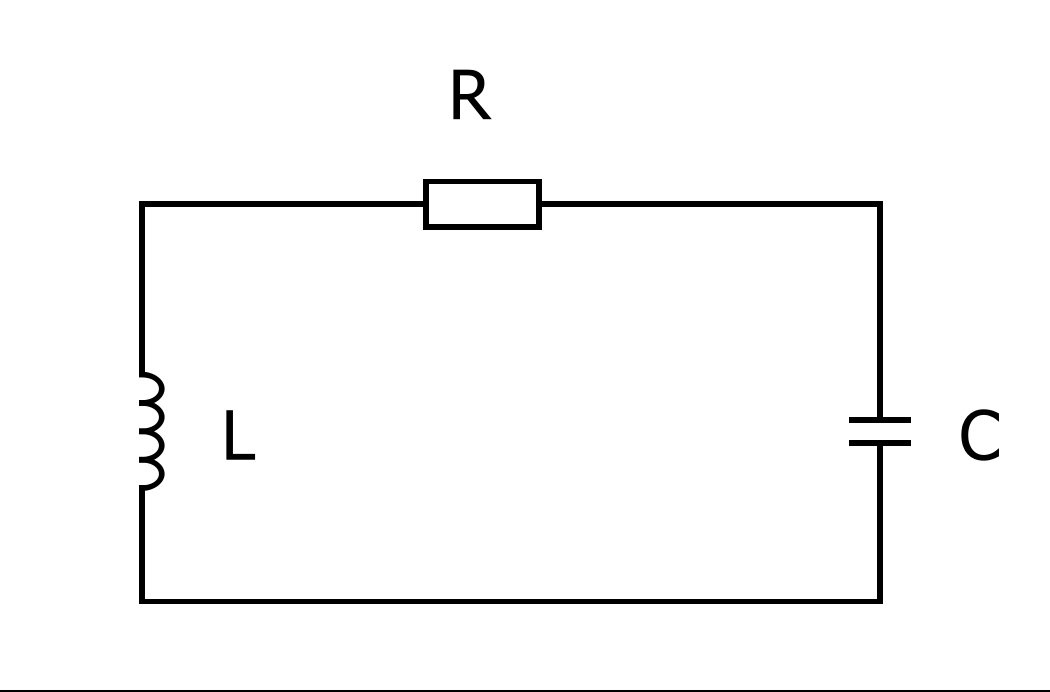
\includegraphics[height= 4cm]{./logos/schwingkreis.png}
  \caption{Einfacher RCL-Kreis bestehend aus einer Spule, einem Widerstand und einem Kondensator}
  \label{fig:rcl}
\end{figure}


\subsection{DGL der gedämpften Schwingung}
Besagte Schwingung lässt sich mithilfe der Kirchhoffschen Summenformel herleiten:

\begin{equation}
  0= \sum_{i=0}^{k} U_i \\
  \iff  0 = U_L + U_R + U_C .
  \label{eqn:kirchhoff1}
\end{equation}

Durch Einsetzen dieser Spannungen in differentieller Form erhält man:

\begin{equation}
  0= L\ddot{Q} + R  \dot{Q} + \frac{1}{C} Q .
  \label{eqn:kirchhoff2}
\end{equation}

Diese Differentialgleichung ist aus der Mechanik bekannt als Bewegungsgleichung eines gedämpften harmonischen Oszillators.
In diesem Fall schwingen Ladungen $Q$ und somit auch der Strom $I$, welcher eine einfacher zu messende und verbreitetere Größe als die Ladung darstellt.
Um eine DGL in $I$ zu erhalten differenziert man \eqref{eqn:kirchhoff2} einfach nach der Zeit und erhält:
\begin{equation}
  0= L \cdot \ddot{I} + R \cdot \dot{I} + \frac{1}{C} \cdot I .
  \label{eqn:kirchhoff3}
\end{equation}


\subsection{Lösung der DGL in drei Fällen}

Die Lösung der DGL \eqref{eqn:kirchhoff3} ist gegeben durch:

\begin{equation}
  I(t) = \symup{exp}(-\beta t) \cdot \Bigl( A \cdot \symup{exp}(i \omega t) B \cdot \symup{exp}(-i \omega t) \Bigr)
  \label{eqn:I(t)}
\end{equation}

mit $\omega = \sqrt{\frac{1}{LC} - \frac{R^2}{4L^2}}$ und $\beta = \frac{R}{2L}$.

Sie unterscheidet sich in 3 Fällen:

\begin{enumerate}
  \item Schwingfall für $\frac{1}{LC} > \frac{R^2}{4L^2}$
  \item Kriechfall für $\frac{1}{LC} < \frac{R^2}{4L^2}$
  \item aperiodischer Grenzfall für $\frac{1}{LC} = \frac{R^2}{4L^2}$
\end{enumerate}

\subsubsection{Schwingfall}
In diesem Fall lässt sich \eqref{eqn:I(t)} schreiben als:
\begin{equation}
  I_s(t)= A_0 \cdot \symup{exp}(-\beta t) \cdot cos(\omega t + \theta)
  \label{eqn:Schwing(t)}
\end{equation}

Es ergibt sich somit eine gedämpfte Schwingung der Umlaufdauer $T= \frac{1}{v} = \frac{2\pi}{\sqrt{1/LC-R^2/4L^2}}$

\subsubsection{Kriechfall}
Da $\frac{1}{LC} < \frac{R^2}{4L^2}$ ergibt sich \eqref{eqn:I(t)}  mit $\tilde{\omega} = \sqrt{\frac{R^2}{4L^2} - \frac{1}{LC}}$ zu:

\begin{equation}
  I_k(t) = A \cdot \symup{exp}((-\beta + \tilde{\omega}) t) + B \cdot \symup{exp}((-\beta - \tilde{\omega}) t)
  \label{eqn:Kriech(t)}
\end{equation}

Je nach Verhältnis $A/B$ kann es bei diesem Stromverlauf bis zu einen Nulldurchgang geben, danach strebt er gegen Null ohne zu schwingen.

\subsubsection{aperiodischer Grenzfall}
Für $\frac{1}{LC} = \frac{R^2}{4L^2}$ reduziert sich \eqref{eqn:I(t)} zu:
\begin{equation}
  I_{ap}(t)= A \cdot \symup{exp}(-\beta t) = A \cdot \symup{exp}\left(- \frac{t}{\sqrt{LC}}\right)
  \label{eqn:AP(t)}
\end{equation}

Dies ist der Extremfall der Dämpfung, d.h. es kann keinen Nulldurchgang geben und der Graph der Funktion nähert sich $I=0$ schneller als im normalen Kriechfall.

\subsection{DGL der erzwungenen Schwingung}
Zwingt man dem RCL-Glied durch zwischenschalten eines Funktionsgenerators ein systemfremdes $U_0(t)$ auf, so erweitert sich \eqref{eqn:kirchhoff2} zu:

\begin{equation}
  L \ddot{I} + R \dot{I} + \frac{1}{C} I = U_0 \cdot \symup{exp}(i \omega t).
\end{equation}

Als Lösung ergibt sich
\begin{equation}
  U_C = \frac{U_O}{1-LC \omega^2 + i\omega RC} \symup{exp}(i\omega t)
  \label{eqn:U_C}
\end{equation}

wobei zu beachten ist, dass $U_C$ eine komplexe Amplitude erhält, deren Betrag
\begin{equation*}
U_0 \sqrt{\frac{(1-LC\omega^2)^2+\omega^2 R^2 C^2}{(1-LC\omega^2)^2 + \omega^2 R^2 C^2}}
\end{equation*}
beträgt.
Die Phase dieser Amplitude ergibt sich zu
\begin{equation*}
\phi(\omega)=\symup{arctan}\left(\frac{-\omega RC}{1-LC\omega^2}\right).
\end{equation*}
Bestimmt man das Maximum der Amplitude so findet man es bei der sog. Resonanzfrequenz, welche der Eigenfrequenz \omega des Schwingkreises entspricht. Es gilt:
\begin{equation}
  U_{C,max} = \frac{1}{\omega RC} U_0
  \label{eqn:Resonanz}
\end{equation}

Man definiert hierbei die Güte $q=\frac{\omega}{\omega_+ - \omega_-}$ wobei $\omega_\pm$ die beiden Frequenzen sind,
bei denen $U_C = \frac{1}{\sqrt{2}} U_{C,max}$, deren Differenz als Breite der Resonanzkurve bezeichnet wird.
Für $R^2/L^2 << \omega^2$ lässt sich die Breite zu $R/L$ nähern.

\subsection{Impedanz}
Bestimmt man den Gesamtwiderstand des RCL-Gliedes, so stellt man fest, dass es sich hierbei um die komplexe Größe
\begin{equation}
  Z = R + i\left(\omega L - \frac{1}{\omega C}\right)
\end{equation}
handelt. Man teilt diesen komplexen Widerstand (Impedanz) in seinen reellen Wirkwiderstand (hier: $R$) und den rein imaginären Scheinwiderstand (hier: $i \left(\omega L - \frac{1}{\omega C}\right)$) ein.
